\documentclass{report}
\title{\Large  Physics 20 - Numerical Integration}
\author{\large Shubh Agrawal, \normalsize\emph{Class of 2022}}
\date{\small October 15, 2018}
\usepackage[a4paper,top=2cm, left=2.5cm,width=13cm,bottom=2cm,right=2.5cm]{geometry}
\usepackage{amsthm, amsmath, amssymb, tipa, graphicx, caption, subcaption, float}

\begin{document}
\maketitle

\subsection*{Introduction}
Several methods of computational numerical integration of basic functions are analyzed. Algorithm-centric Python programs are implemented for trapezoid approximation and Simpson's method; their error's dependence on contained variables is graphically studied through progressive simulations, and is used in improving code to provide values within specified error bounds. Predefined systems of integration, notably Romberg's method,  are also taken up in comparison. Source code is available as attachment (\texttt{Assignment2.py}).
\subsection*{Extended Simpson's Formula}
Here, the extended Simpson's formula for integration approximation is derived. The orders of the local and global errors are also derived.
\\\\
The Simpson's rule is defined for one interval as follows:
$$I_{\text{simp}}\equiv H\Big(\frac{f(a)}{6}+\frac{4f(c)}{6}+\frac{f(b)}{6}\Big)$$
where $H =b-a$, and $c=(a+b)/2$. Writing $f(x)$ as a Taylor sum about $a$ and integrating each side,
\begin{align*}
	f(x) &= f(a)+ f'(a)(x-a)+\frac{f''(a)}{2!}(x-a)^2+\frac{f'''(a)}{3!}(x-a)^3+\cdots\\
	&=f(a)+f'(a)(x-a)+\frac{f''(a)}{2!}(x-a)^2+\frac{f'''(a)}{3!}(x-a)^3 + \frac{f''''(\eta)}{4!}(x-a)^4 &\text{with $x, \eta \in[a,b]$}\\
\end{align*}
Now, $$	I=f(a)H+f'(a)\frac{H^2}{2!}+f''(a)\frac{H^3}{3!}+f'''(a)\frac{H^4}{4!}+f''''(\eta)\frac{H^5}{5!}$$
Approximating using the Taylor series expression and putting $c-a=H/2$ and $b-a=H$,
\begin{align*}
	I_{\text{simp}}&= \frac{f(a)}{6}H+\frac{4f(c)}{6}H+\frac{f(b)}{6}H\\
	&=\frac{f(a)}{6}H+
	\Big(\frac{4f(a)H}{6}+f'(a)\frac{4H^2}{6\cdot 2}+\frac{f''(a)}{2!}\frac{4H^3}{6\cdot 4}+\frac{f'''(a)}{3!}\frac{4H^4}{6\cdot 8}+ \frac{f''''(\eta)}{4!}\frac{4H^5}{6\cdot 16} \Big)
	\\&\qquad+\Big( \frac{f(a)H}{6}+\frac{f'(a)H^2}{6}+\frac{f''(a)H^3}{6\cdot 2!}+\frac{f'''(a)H^4}{6\cdot 3!}+ \frac{f''''(\eta)H^5}{6\cdot 4!}\Big)\\
	&=f(a)H+f'(a)\frac{H^2}{2!}+f''(a)\frac{H^3}{3!}+f'''(a)\frac{H^4}{4!}+f''''(\eta)\frac{5H^5}{24\cdot4!}
\end{align*} 
Then, $I - I_{\text{simp}} = f''''(\eta)\frac{H^5}{5!} - f''''(\eta)\frac{5H^5}{24\cdot4!} \propto H^5$. Thus, it is derived that the local error under Simpson's Rule is of the fifth order, or $I= I_{\text{simp}} + O(H^5)$.

For deriving the \emph{extended} Simpson's formula, the integral interval $(a,b)$ is divided into $N$ subintervals. However, it is noted that, in comparison to the trapezoid rule analysis, there are actually $2N$ divisions as each interval $(a',b')$ is broken into two by $c'$. So, taking $h_N=(b-a)/N$, and $x_0=a, x_1= a +h_N/2, x_2= a+h_N, \dots, x_{2N}=b$,
\begin{align*}
	\int_a^b f(x) \, dx &= \int_{x_0}^{x_2} f(x) \, dx + \int_{x_2}^{x_4} f(x) \, dx + \cdots + \int_{x_{2N-2}}^{x_{2N}} f(x) \, dx \\
	&\simeq h_N (\frac{f(x_0)}{6}+\frac{4f(x_1)}{6}+\frac{f(x_2)}{6}) + (\frac{f(x_2)}{6}+\frac{4f(x_3)}{6}+\frac{f(x_4)}{6})+ \cdots + (\frac{f(x_{2N-2})}{6}+\frac{4f(x_{2N-1})}{6}+\frac{f(x_{2N})}{6})\\
	&=\frac{h_N}{6}\Big(f(x_0)+4f(x_1)+2f(x_2)+4f(x_3)+ \cdots +2f(x_{2N-2}) + 4f(x_{2N-1}) + f(x_{2N})\Big)
\end{align*}
The global error of the extended Simpson approximation would be
 $$f''''(\eta')\frac{5h^5_N}{24\cdot 4!}N\propto h_N^5\frac{(b-a)}{h_N}\propto h_N^4\qquad \text{with } \eta'\in[a,b]$$
 
 Thus, the global error of the Simpson expression of the fourth order, or, $O(h_N^4)$.
 \pagebreak
\subsection*{Convergence rate for Trapezoid and Simpson's Formulas}
A Python method was implemented to run models determining error bounds in integration approximations for either method. These models varied in the minimum and maximum subintervals studied. A overlaying graph was also plotted to not the difference of order between trapezoid (\emph{second order}) and Simpson expressions (\emph{fourth order}). The plots are plotted in log-log space to linearize the curve.
\begin{figure}[H]
	\centering
	\includegraphics[width = 0.8\textwidth]{se.png}
	\label{trapezoid1}
	\caption{Convergence of error for trapezoid approximation of $\int_{0}^{1}e^x$. Number of subintervals $N$ ranges from 100 to 500.}
\end{figure}
\begin{figure}[H]
	\centering
	\includegraphics[width = 0.8\textwidth]{ss.png}
	\label{trapezoid2}
	\caption{Convergence of error for trapezoid approximation of $\int_{-\pi/2}^{\pi/2}\cos x$. Number of subintervals $N$ ranges from 1000 to 100000.}
\end{figure}
\begin{figure}[H]
	\centering
	\includegraphics[width = 0.8\textwidth]{te.png}
	\label{simpson1}
	\caption{Convergence of error for Simpson approximation of $\int_{0}^{1}e^x$. Number of subintervals $N$ ranges from 100 to 500.}
\end{figure}
\begin{figure}[H]
	\centering
	\includegraphics[width = 0.8\textwidth]{ts.png}
	\label{simpson2}
	\caption{Convergence of error for Simpson approximation of $\int_{0}^{\pi}\sin x$. Number of subintervals $N$ ranges from 100 to 10000. Note how the rate of error decrease seems to decay to constant error beyond third order $N$. }
\end{figure}
\begin{figure}[H]
	\centering
	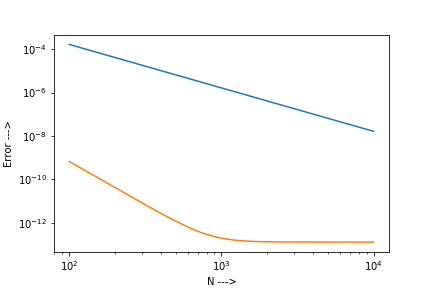
\includegraphics[width = 0.8\textwidth]{both.png}
	\label{both}
	\caption{Legend: \emph{orange} $\leftrightarrow$ Simpson; \emph{blue} $\leftrightarrow$ Trapezoid. \\Convergence of error for both approximations of integral of $\sin x$ from 0 to $\pi$. Number of subintervals $N$ ranges from 100 to 10000. Note that the Simpson error bound is greatly smaller than the trapezoid error. Note how the magnitude of slope for Simpson is higher than that of the trapezoid method for the precise part, indicating that the former is a superior formula.}
\end{figure}

\begin{figure}[H]
	\centering
	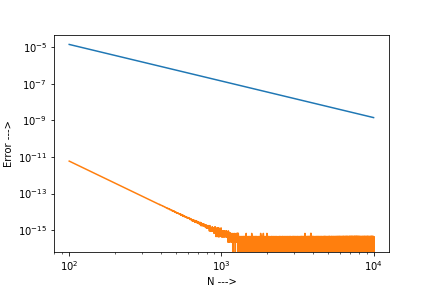
\includegraphics[width = 0.8\textwidth]{both1.png}
	\label{both1}
	\caption{Legend: \emph{orange} $\leftrightarrow$ Simpson; \emph{blue} $\leftrightarrow$ Trapezoid. \\Convergence of error for both approximations of integral of $e^x$ from 0 to 1. Number of subintervals $N$ ranges from 1000 to 100000. Note how the floating point imprecision is even more evident when the integral value is a bounding value too ($e -1$).}
\end{figure}


In Figures 4, 5, and 6, it is noted that the Simpson error seems to not decrease beyond a certain number of simulations. Floating point precision limits (the innate storage precision of \texttt{float} values in computer memory) do not allow greater accuracy, or simply put, the unit cannot measure the returned values of the function accurately to say anything conclusive. It is also notable that this is only observed in our Simpson plots at high $N$, as the trapezoid method gives several order of magnitudes (~5) larger errors, which do not reach the limits of memory precision. The limit might be reachable by increasing the order of magnitude of $N$ by the said order (~5), which would take high computational power and time complexity, and is not therefore demonstrated here.

\subsection*{Comparison with \texttt{scipy.integrate} module}
 Similar analysis was carried out on the \texttt{quad} and \texttt{romberg} functions of the \texttt{scipy.integrate} module. Note that these two do not take number of subintervals as arguments and, thus, give a constant error bound (represented as straight lines parallel to the $Y$-axis on the graphs below) for all $N$. 
 
 The integral $\int_{0}^{1} e^x$ is analyzed in all cases; wherever applicable, the number of divisions are taken fairly large to get lower error scales.
\begin{figure}[H]
	\centering
	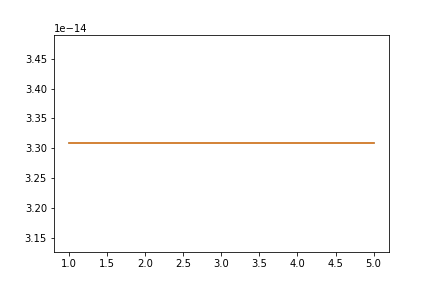
\includegraphics[width = 0.8\textwidth]{scipy1.png}
	\label{scipy1}
	\caption{Romberg method error order (in linear space)}
\end{figure}
\begin{figure}[H]
	\centering
	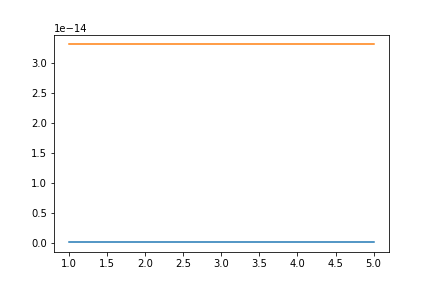
\includegraphics[width = 0.8\textwidth]{scipy2.png}
	\label{scipy2}
	\caption{\texttt{romberg} (\emph{orange}) method versus \texttt{quad} (\emph{blue}) method (in linear space)}
\end{figure}
\begin{figure}[H]
	\centering
	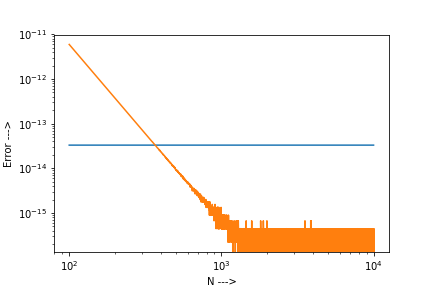
\includegraphics[width = 0.8\textwidth]{scipy3.png}
	\label{scipy3}
	\caption{\texttt{romberg} method (\emph{blue}) versus Simpson's formula (\emph{orange}) (in logarithmic space), for $N$ from 100 to 10000. Note that Simpson's error does (seem) to go below the romberg error, but, due to floating precision, it is irregular and imprecise.}
\end{figure}
\begin{figure}[H]
	\centering
	\includegraphics[width = 0.8\textwidth]{scipyN.png}
	\label{scipy3.5}
	\caption{\texttt{romberg} method (\emph{blue}) versus Simpson's formula (\emph{orange}), for $N$ from 100 to 5000, for integral of $\sin x$ over 0 to $\pi$. Note how the Simpson error does not oscillate when the actual value of integral is not a bounding (irrational-like) float value. (Here it is simply 2.0)}
\end{figure}
\begin{figure}[H]
	\centering
	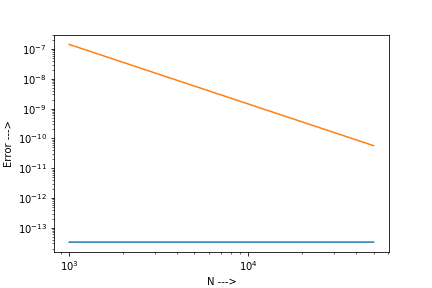
\includegraphics[width = 0.8\textwidth]{scipy4.png}
	\label{scipy4}
	\caption{\texttt{romberg} (\emph{blue}) method versus trapezoid formula (\emph{orange}), range of $N$ from 1000 till 50000. Note the large difference in order of magnitudes.}
\end{figure}
\begin{figure}[H]
	\centering
	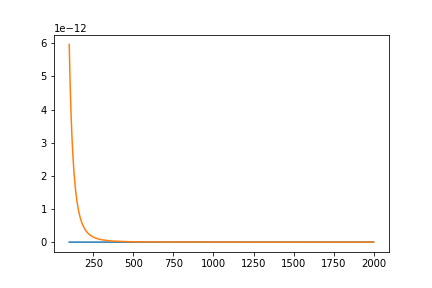
\includegraphics[width = 0.8\textwidth]{scipy5.png}
	\label{scipy5}
	\caption{\texttt{quad} method (\emph{blue}) versus Simpson's formula (\emph{orange}), for $N$ from 200 to 2000, in linear space, as quad errors are not always positive.}
\end{figure}
It is noted that, as expected, the \texttt{scipy.integrate} methods approximate the integral more accurately and faster (less memory manipulated) for practical purposes. Increasing $N$ does cause the Simpson error to converge towards 0, yet due to floating precision, it is ineffective as compared to \texttt{quad} as all values, and \texttt{romberg} at lower values of $N$ (which are usually used in fast computation).
\end{document}